% !TeX spellcheck = en_GB
\begin{figure}
  \setlength{\unitlength}{\textwidth}
  \begin{picture}(1,0.3)(-0.02,0)
          
    \put(0.025,0.04){\includegraphics[width=0.5\unitlength]{../FnP/gnuplot/p_max.eps}}
    \put(0.6,0.04){\includegraphics[width=0.5\unitlength]{../FnP/gnuplot/p_2_p_max.eps}}
        
    \put(0.54,0.07){ \rotatebox{90}{$\displaystyle\massdamp$ \scriptsize{at max power}} }
    \put(-0.07,0.16){$\displaystyle\frac{P_{max}}{\rho \mathcal{A}U^3 }$}
    % \put(0.73,0.00){ $\displaystyle\frac{c}{\rho\mathcal{A}U}$}

    \put(0.25,0.00){\massstiff}
    \put(0.85,0.00){\massstiff}
   
    \put(0.058,0.07){\small(a)}
    \put(0.634,0.07){\small(b)}
      
    \end{picture}

    % \caption{Comparison of DNS data. (a) Maximum power obtained using
    %   a 3 point localised quadratic fitting as a function of
    %   \massstiff. (b) \massdamp as a function of \massstiff at maximum
    %   power}

    \caption{(a) Maximum power, and (b) the value of \massdamp\ 
        where maximum power occurs, as functions of \massstiff,
        extracted from the DNS data presented in figure
        \ref{fig:qss_fsi}. The maximum power asymptotes to an upper
        value with increasing \massstiff, while the value of \massdamp\
        where maximum power occurs is relatively insensitive to
        \massstiff.}

    \label{fig:max_power}
\end{figure}

 %vspace{10cm}
